\documentclass[12pt]{article}
%\usepackage{amsmath,amsfonts,amssymb}
\usepackage{epsf}
\usepackage{graphicx,wrapfig,lipsum}
\RequirePackage{amsfonts,amssymb,amsmath,amscd,amsthm}
\usepackage{epsfig,tabularx,graphicx,float}
\usepackage{graphicx,parallel}
\usepackage{a4wide}
\graphicspath{ {C:/Users/RAJ/OneDrive/sem_10/Project/Graphs/}}
\linespread{1.5}
\begin{document}
%First page of the document	
\thispagestyle{empty}
\begin{center}
\textrm{\textbf{\large Brief Study of Censoring  process using Exponential Distribution}}
\end{center}
\vspace{0.5cm}
\begin{center}
A THESIS \\
SUBMITTED TO THE\\
NATIONAL INSTITUTE OF TECHNOLOGY, ROURKELA\\

\includegraphics[width=0.4\textwidth]{NitLogo.jpg}\\
IN THE PARTIAL FULFILMENT\\
FOR THE DEGREE OF \\
MASTER OF SCIENCE IN MATHEMATICS\\
BY\\
RAJ KUMAR\\
UNDER THE SUPERVISION OF\\
Dr. MANAS RANJAN TRIPATHY \\
%\end{center}
%\vspace{3cm}
%\begin{figure}[htbp]
%\begin{center}
%\baselineskip=20pt
\nopagebreak
DEPARTMENT OF MATHEMATICS\\
NATIONAL INSTITUTE OF TECHNOLOGY ROURKELA\\
MAY, 2016
\end{center}
%\end{figure}





%Second page of the document
\newpage
\pagenumbering{roman}
\begin{center}
\textbf{\Large CERTIFICATE}
\end{center}
\vspace{2cm}
\begin{quote}
This is to certify that the thesis entitled  \textbf{\textit {Brief Study of Censoring process using Exponential Distribution}}, which is being submitted by Raj Kumar in the Department of Mathematics, National Institute of Technology, Rourkela, in partial fulfilment for the award of the degree of Master of Science, is a record of bonafide review work carried out by him in the Department of Mathematics under my guidance. He has worked as a project student in this Institute for one year. In my opinion the work has reached the standard, fulfilling the requirements of the regulations related to the Master of Science degree. The results embodied in this thesis have not been submitted to any other University or Institute for the award for any degree or diploma.
\end{quote}
\begin{flushleft}
	Rourkela  \hfill Dr. Manas Ranjan Tripathy\\
	May 13, 2013\hfill Professor,N.I.T Rourkela
\end{flushleft} 




%Third page of the document
\newpage
\vspace{0.5cm}
\begin{center}
\textbf{\Large Preface}
\end{center}
The precious debt of learning is a debt that is difficult to pay, only gratitude can be felt. I feel great pride and privilege in expressing my heartfelt, deep sense of gratitude and profound thanks to my esteemed Major Advisor Dr. Manas Ranjan Tripathy, Professor , Department of Mathematics for their insight advise, keen interest, valuable suggestions, constructive criticism, ever available and untiring help, constant encouragement during the period of study.\\
It is prerogative to have worked under his supervision. My work under his will always remain an unforgettable experience of my life.I am also thankful to the laboratory of Department of Mathematics for their kind helps during the research work.\\
I pay my overwhelming reverence, regards and love towards my family members for their tacit-orts, un-inching cooperation and affection for me.\\
I extend my eternal gratitude to those learned souls, many known and unknown hands
who are always guiding me towards the right goal.\\
I express my happiness at being able to get my professional knowledge from N.I.T,
Rourkela ,Odisha and feel proud at being part of this institute. Last but not the least,I thank Almighty God for giving me patience and strength to overcome the difficulties which crossed my way in accomplishment of this endeavor.
\vspace{2cm}
\begin{flushleft}
Rourkela  \hfill Raj Kumar\\
May 13, 2013\hfill 411ma5058
\end{flushleft}




%Fourth page of the document
\newpage
\vspace{0.5cm}
\begin{center}
	\textbf{\Large ABSTRACT}
\end{center}
 Censoring holds a prominent field in medical diagnosis and engineering,economics and many fields.Initially the process of censoring was used for the process of deciding the lifetime of the statistic where the the data is missing. In the following thesis we will study the process of censoring using exponential distribution and will apply the results to derive various estimation on Exponenital distribution and will derive the results related to it such as parameter estimation of exponential distribution, inference based results and will derive the basic results related to the exponential distbribution such as cumulative distribution function(CDF),survivor function ,entropy,and many other results.of pdf and cdf, asymptotes, quantile function, moment, extreme
 values, reliability, mean, median, mode, moment generating function, order statistics,Renyi and Shannon Entropy, bivariate generalizations and Maximum likilihood estimator (MLE). We also propose some theorems pertaining to moment of these distributions.




%5th page of the document
\newpage
\vspace{0.5cm}
\begin{center}
\textbf{\Large CONTENTS}
\end{center}
\begin{description}
     \item[1.] \textbf{Introduction and Motivation}
       \begin{description}
         \item 1.1 Introduction to censoring
         \item 1.2 Censoring process.
         \item 1.3  Exponential Distribution
         \item 1.4 Statistic related to exponential distribution 
       \end{description}
     \item[2.] \textbf{Estimation of parameters using Type-2}
      \begin{description}
       \item 2.1 
       \item 2.2
       \item 2.3
       \item 2.4 
       \item 2.5 
      \end{description}
     \item[3.] \textbf{Progressive Censoring in Exponential distribution}
      \begin{description}
       \item 3.1 
       \item 3.2 
       \item 3.3 
       \item 3.4 
      \end{description}
     \item[4.] \textbf{Hybrid censoring in Exponential Distribution}
      \begin{description}
	   \item 4.1 
	   \item 4.2 
	   \item 4.3 
	   \item 4.4 
      \end{description}
     \item[5.] Conclusion and Future work
      \begin{description}
	   \item[5.1] description
	   \item[5.2] description
      \end{description} 
\end{description}







\newpage
\setcounter{page}{1}
\pagenumbering{arabic}
\vspace{0.5cm}
\begin{flushleft}
\textbf{\Large Chapter 1}
\end{flushleft}
\vspace{0.1cm}
\begin{flushleft}
\textbf{\Large Preliminaries and Introduction}
\end{flushleft}
\vspace{0.2cm}
\noindent \textbf{\large 1.1. Introduction to Censoring}\\
\vspace{0.2cm}
In reliability and Lifetime data analysis when the data is incomplete than various procedures are applied to get the estimate of the statistic of the given dataset.One of the procedure is known as censoring.\\
Censoring is defined as the process in which the statistic are derived from the incomplete data using the appropriate methods. Censoring can be broadly divided into four main parts as per given.\\
1) Type -I Censoring process.\\
2) Type -II Censoring process.\\
3) Progressive Censoring.\\
4) Hybrid Censoring.\\

\textbf{Type-1 Censoring}\\
 \quad Let Consider n random variables given by $X_{1},X_{2},X_{3},...,X_{n}$ such that cumulative distributive function exists.If we apply a fixed time $t_{c}$ after which gathering of data is stopped  than it is known as the type-1 censoring.Here pre assigned time is $t_{c}$.
 In following process we will observe on $ T_{1},T_{2},T_{3},...,T{r}$ such that $r<n$ and
 and we will have
\[
T_{i}= 
\begin{cases}
\   T_{i},       & \text{iff }\quad T_{i}\geq t_{c}\\
    t_c,         & \text{iff}\quad T_{i}< t_{c}
\end{cases}
\]

\textbf{Type-2 Censoring}\\
 \quad Let consider there are n random variables given by $X_{1},X_{2},X_{3},...,X_{n}$
 such that the cumulative distribution function exists for the given random variables.There exists a r such that $r<n $ and if we will choose r values out of n  random variables in an ordered ways such that $X_{1}<X_{2}<X_{3}<...<X_{n}$ and
 now taking out only r values than the full ordered sample will be given by the\\
 $
 Y_{1}=X_{1}\\
 Y_{2}=X_{2}\\
 Y_{3}=X_{3}\\
  ..........\\
 Y_{r}=X_{r}\\
 $
 
 \textbf{Progressive Censoring}\\
 Let $X_{1},X_{2},X_{3},...,X_{n}$ be independent and identically distributed (i.i.d.) random lifetimes of n items. A progressive type-II right censored sample can be obtained in the following way: at the time of the first failure, noted $X_{1:m:n}$,$r_{1}$ surviving items are removed at random from the n−1 remaining surviving items, at the time of the next failure, noted $X_{2:m:n}$, r2 surviving items are re-moved at random from the $n-r_{1} - 2$ remaining items, and so on. At the time of the $m_{th}$ failure, all the remaining $r_{m}$=n-m-r1-...-$r_{m}$−1 surviving items are censored.
 
 \textbf{Hybrid Censoring}\\
 A hybrid censoring sampling scheme can be described as follows. Each unit in a randomly selected sample of n units is subjected to a life test under identical environmental conditions. The lifetimes of the sample units are independent and identically distributed (i.i.d) random variables. The test is terminated when a pre-chosen number R, out of n items have failed or when a pre-determined time, T, on test has been reached. It is also assumed that the failed items are not replaced. A schematic illustration is depicted in Figure 1, when y1:n < : : : <
 yR:n denote the observed failure times if yR:n < T and $y_{1:n}<...<y_{d:n}$ denote the observed failure times if $y_{d:n} < T, d < R$ and the $(d + 1)^{th}$ failure does not take place before time point T.


\newpage
\begin{flushleft}
\textbf{\Large Exponential Distribution and its properties}\\
\end{flushleft}
 Let consider a random varibale than X than a two-parameter exponential distribution is given by the following formulae\\
\begin{Parallel}[v]{0.48\textwidth}{0.48\textwidth}
	\ParallelLText{ 
		\[
		f(x)= 
		\begin{cases}
		\frac{1}{\sigma} e^{\frac{-(x-\mu)}{\sigma}}      & \text{iff } -\infty<\mu<\infty,\\
		      \hspace{1.5 cm}x>\mu\\
		0,         & \text{otherwise} 
		\end{cases}
		\] }
	\ParallelRText{
		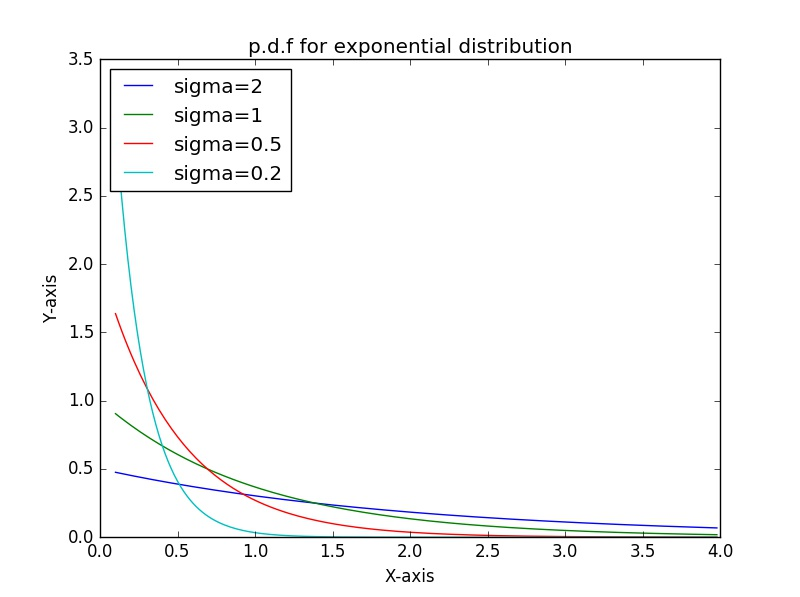
\includegraphics[width=0.4\textwidth]{pdf.jpeg}
	}
\end{Parallel}
     

The cumulative distribution function for two parameter function will be given by the following
%\begin{Parallel}
\begin{Parallel}[v]{0.48\textwidth}{0.48\textwidth}
\ParallelLText{	
\[
F(x)=
\begin{cases}
     1-e^{{\frac{-(x-\mu)}{\sigma}}} &\text{iff} -\infty<\mu<\infty,\\      \hfill x>\mu\\
     0                             &\text{otherwise}
\end{cases}
\]
}
\ParallelRText{
	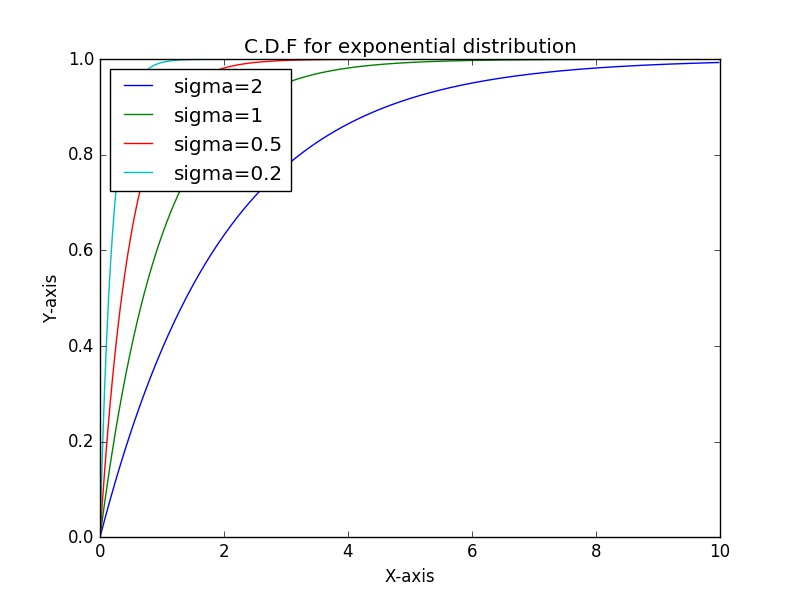
\includegraphics[width=0.4\textwidth]{cdf.jpeg}
	}
\end{Parallel}
Here the mean of the exponential distribution is first moment generating function and can be calculated using following function\\
\begin{center}
$E(x)=\int_{-\infty}^{\infty}x*f(x)dx$\\
$=\int_{-\infty}^{\infty}x*\frac{1}{\sigma}e^{\frac{-(x-\mu)}{\sigma}}$\\
$=\mu$\\
\end{center}
Variance of any distribution measures the spreadness of the the given distribution for exponential distribution the variance can be found using the following
\begin{center}
	$Var(x)=E(X^2)-E(X)^2$\\
	$=\int_{-\infty}^{\infty} x^2*\frac{1}{\sigma}exp(\frac{-(x-\mu)}{\sigma}) dx -\int_{-\infty}^{\infty} x*\frac{1}{\sigma}exp(\frac{-(x-\mu)}{\sigma})dx$\\
	$=\sigma^2$
\end{center}

The above statistic can be derived from the moment generating functions for which the general forumala for piecewise continous function is given by the
\begin{center}
	$E(X^n)=\int_{-\infty}^{\infty} x^n f(x)dx$
\end{center}
for the exponential distribution the formulation will be given by the following
\begin{center}
	$E(X^n)=\int_{-\infty}^{\infty} x^{n}\frac{1}{\sigma}e^{\frac{-(x-\mu)}{\sigma}}dx$\\
	$E(X^n)=n!*\sigma^n$
\end{center}

For any probabilistic function the median value as the most middle value occuring and can be calculated using 
\begin{center}
	$P(X<=x)=\frac{1}{2}$\\
\end{center}
calculating the median for the exponential distribution using following formulae we will have the value given by
\begin{center}
	$x=\log(2)\sigma$
\end{center}
 Moment generating function is defined by the following formula
 \begin{center}
 	$M(t)=E(e^{tx})$
 \end{center}
 for the exponential distribution the M.G.F can be found by using the following formuale
 \begin{center}
 	$M(t)=E(e^{tx})$\\
 	$=\int_{-\infty}^{\infty} e^{tx}f(x) dx$\\
 	$\int_{\mu}^{\infty} e^{tx} \frac{1}{\sigma} exp(\frac{-(x-\mu)}{\sigma}) dx$\\
 	$M(t)=\frac{1}{\sigma (\frac{1}{\sigma}-t)} e^{\frac{\mu}{\sigma}} e^{-\mu(\frac{\mu}{\sigma}-t)} $\\
 \end{center} 
 
 P.G.F(probability generating function) For a continous distribution p.g.f can be defined as
 \begin{center}
 $P(s)=\int_{-\infty}^{\infty} s^x f(x) dx$
 \end{center}
 for the exponential distribution the p.g.f will be given by the following function which will simplify to the following formula
 \begin{center}
 $=\int_{\mu}^{\infty} s^{x} \frac{1}{\sigma} e^{\frac{-(x-\mu)}{\sigma}} dx$\\
 $=\int_{\mu}^{\infty} e^{x logs} \frac{1}{\sigma}e^{\frac{-(x-\mu)}{\sigma}} dx$\\
 	$P(s)=\frac{1}{\sigma (\frac{1}{\sigma}-\log{s})} e^{\frac{\mu}{\sigma}} e^{-\mu(\frac{\mu}{\sigma}-\log{s})} $\\
 
 \end{center}
 \begin{flushleft}
 \textbf{Estimation of parameter for Single parameter exponential Distribution}
\end{flushleft}
 In statistics estimation of parameter is used for finding the most appropriate value for the given distribution to estimate its parameter. Most commonly used methods are given by the following\\
 \begin{description}
 \item[1.] \textbf{Methods}
 \begin{description}
 	\item[1.1] Maximum Likelihood estimator
 	\item[1.2] Method of moments
 \end{description}
 \end{description}
 \textbf{Maximum Likelihood estimator}
 Considering we have a single  parameter exponential distribution given as
   \[
   f(x)= 
   \begin{cases}
   \   \frac{1}{\sigma} e^{\frac{-(x-\mu)}{\sigma}}      & \text{iff } x>\mu\\
   0,         & \text{otherwise} 
   \end{cases}
   \] 
  than the moment generating function will be given by the following
  \begin{center}
  	$f(x_{i})= \frac{1}{\sigma} e^{\frac{-(x_{i}-\mu)}{\sigma}}$\\
  	$\prod f(x_{i})=\prod  \frac{1}{\sigma} e^{\frac{-(x_{i}-\mu)}{\sigma}} $
  	\begin{flushleft}
  	let consider product of all f(x) is denoted by L and parameter is sigma than
  	\end{flushleft}
  	$L(\mu,\sigma)=\prod_{i=1}^{n} \frac{1}{\sigma} e^{\frac{-(x_{i}-\mu)}{\sigma}}$\\
  	$=\frac{1}{\sigma^n} e^{\frac{-1}{\sigma} (\sum_{i=1}^{n} x_{i}-\mu)}$\\
  		\begin{flushleft}
  			Taking logarithm on the both side we will have the following
  		\end{flushleft}
  	$-n\log{\sigma}-\frac{1}{\sigma}(\sum_{i=1}^{n} x_{i}-\mu)$
  	\begin{flushleft}
  		Differntitating with respect to the parameters we can get the estimate of the full data for the parameters.
  	\end{flushleft}
  	$\hat{\mu}=min(x_{i})$\\
  	$\hat{\sigma}=\frac{1}{n} \sum_{i=1}^{n}(x_{i}-\mu)$
  	
  \end{center}
 
 \textbf{Methods of moment}
 In Statistics alternative of the maximum likelihood estimator is given by the methods of moments.Let consider there are n i.i.d random variables than the estimation of parameter can be done using the moments. Moments required to estimate parameter will depend on the number of parameter.For two parameter exponential distribution the moment can be found as per given.
  
 

In the censoring process many function are being used which gives better insight of the working of the function for the given
Let consider a probability density function given by $f(x)$ than the surival function is given by the than survival function will be given by following using the moment generating function.\\
\begin{center}
	$E(e^{tx})=\int_{-\infty}^{\infty} e^{tx} f(x) dx$\\
	$=\int_{\infty}^{\infty} e^{tx} e^{\frac{-(x-\mu)}{\sigma}} dx$\\
	$=e^{\mu t}\frac{1}{(\sigma*(\frac{1}{\sigma}-t))}$
\end{center}
using the following value we will have first and second moment as per given 
\begin{center}
	$\mu^{1}=\mu+\sigma$\\
	$\mu^2=\mu+2\mu \sigma +2\sigma^2$
\end{center}
Hence from here we will have following result
\begin{center}
	$\mu_{X}=\mu+\sigma$\\
	$\sigma_{x}=\sigma$\\
\end{center}

\newpage
\textbf{Survivor function}
  Let consider random variable T and the probability density function $f(x)$ whose
  cumulative distribution function is given by $F(x)$ than the survivor function is 
  defined as following
 \begin{center}
 	$S(x)=P(T>t)=\int_{t}^{\infty} f(x) dx$\\
 	$=1-F(t)$
 \begin{flushleft}
 	for exponential distribution survivor function is given by
 \end{flushleft} 
 \end{center}
\begin{Parallel}[v]{0.48\textwidth}{0.48\textwidth}
	\ParallelLText{ 
		\[
		S(x)= 
		\begin{cases}
		e^{\frac{x-\mu}{\sigma}}      & \text{iff } -\infty<\mu<\infty,x>\mu\\
		0,         & \text{otherwise} 
		\end{cases}
		\] }
	\ParallelRText{
		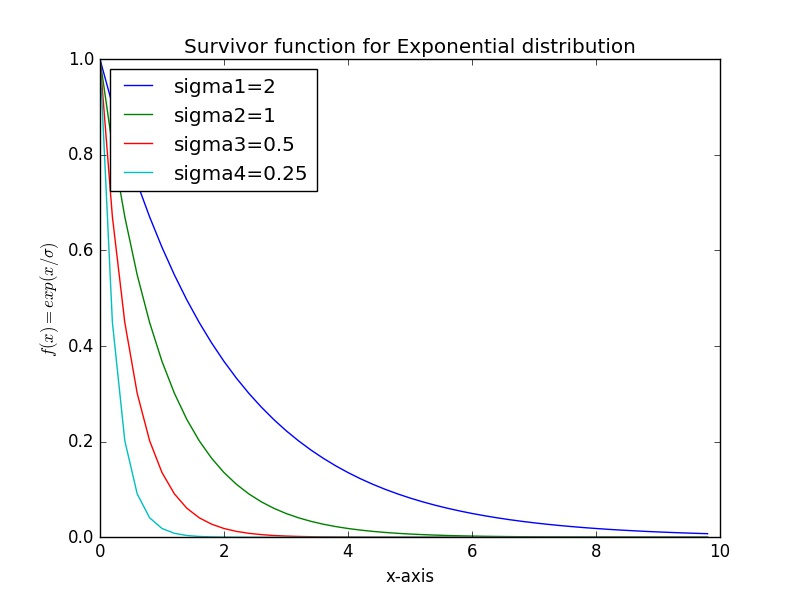
\includegraphics[width=0.4\textwidth]{survivor.jpeg}
	}
\end{Parallel}

 A basic quantity, fundamental in survival analysis, is the hazard function.This function is also known as the conditional failure rate in reliability,the force of mortality in demography, the intensity function in stochastic processes, the inverse of the Mill’s ratio in economics, or simply as the hazard rate. The hazard
 rate is defined by\\
 \begin{center}
 	$h(x)=\lim\limits_{x-0}\frac{Pr(x<X<x+\delta x|X\geq x)}{\delta x} $\\
 \end{center}
 If $X$ is a continuous random variable, then,\\
 \begin{center} 
 	$h(x)=f(x)/S(x)=-d(S(x))/dx $\\
 \end{center}
 and a related quantity is also defined as the cumulative hazard function given by
 \begin{center}
 	$H(x)=\int_{0}^{x} h(u)du$
 \end{center} 
 In case of exponential distribution the hazard function and cumulative hazard function is given by the following function
 \begin{Parallel}[v]{0.48\textwidth}{0.48\textwidth}
 	\ParallelLText{ 
 		\[
 		f(x)= 
 		\begin{cases}
 		\frac{1}{\sigma}      & \text{iff } -\infty<\mu<\infty,x>\mu\\
 		0,         & \text{otherwise} 
 		\end{cases}
 		\] }
 	\ParallelRText{
 		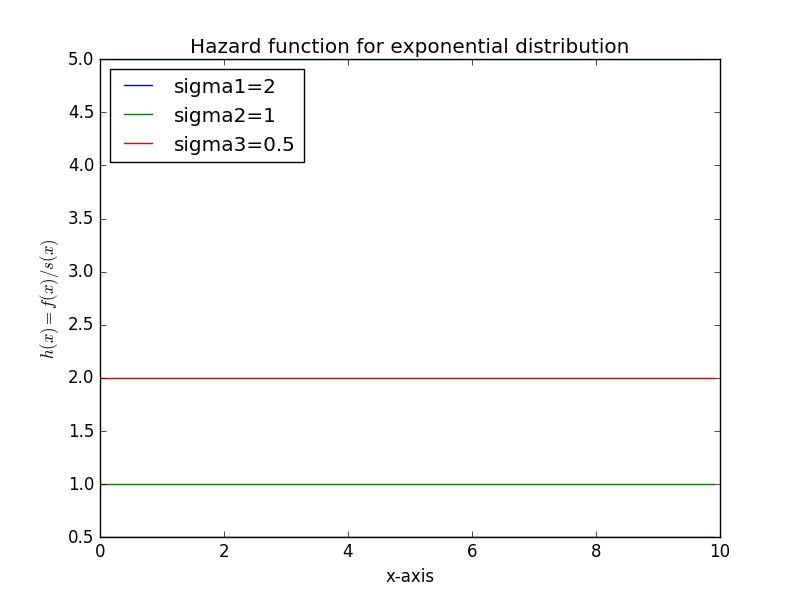
\includegraphics[width=0.4\textwidth]{hazard.jpeg}
 	}
 \end{Parallel}
 \begin{flushleft}
 	Cumulative hazard function will be the integration of the hazard function
 \end{flushleft}
  
\begin{Parallel}[v]{0.48\textwidth}{0.48\textwidth}
	\ParallelLText{ 
		\[
		f(x)= 
		\begin{cases}
		\frac{x}{\sigma}      & \text{iff } -\infty<\mu<\infty,x>\mu\\
		0,         & \text{otherwise} 
		\end{cases}
		\] }
	\ParallelRText{
		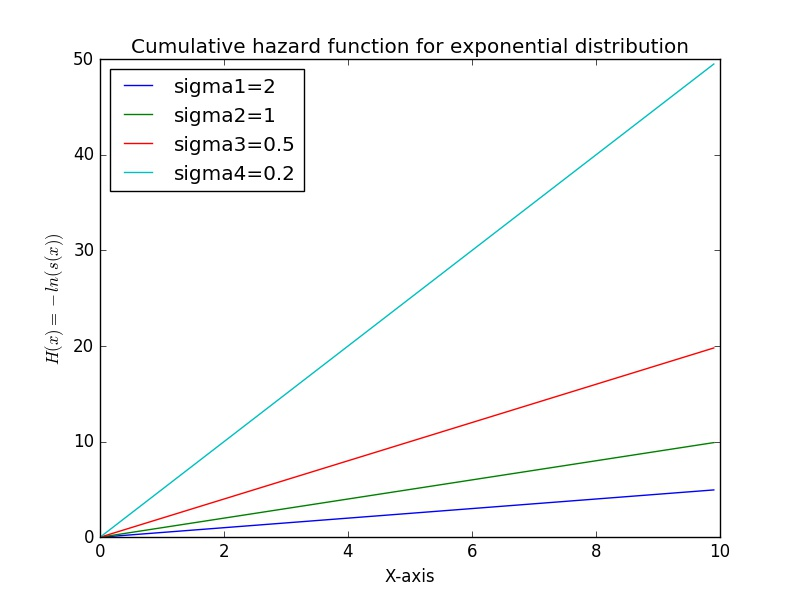
\includegraphics[width=0.4\textwidth]{cumulative_hazard.jpeg}
	}
\end{Parallel}


\newpage
\begin{flushleft}
	\textbf{\Large Chapter 2}
\end{flushleft}
\vspace{0.1cm}
\begin{flushleft}
	\textbf{\Large Type-I and Type-II censoring and estimation of parameter}
\end{flushleft}
\vspace{0.2cm}
Let consider a problem in which we have to check the reliability of n given test-items drawn randomly from a population.we have to determine whatever failure
rate is acceptable or not.In given test scenario we will fix the time T to test the running time to see if they fail or survive .Thus the data obtained will be censored Type-1 data.
During the duration of T hours we observe r failures ($0\leq r \leq n$).The exact failure time are $t_{1},t_{2},t_{3},...,t{r}$ and there are (nor) units which survived the hour test without any failure. Here we T is pre-fixed and r is a random number.Censoring process done in this way is known as the "right censoring"
since the failures are to the right are missing(larger values than T)

Let consider another situation in which number of failures are predecided let sat r.
In the following scenario testing time is not available.Let consider we have n=200
and we want to see 23 percent of them fail than r=50 but her T is unknown until the $50^th$ failure and the following type of censoring process is known as Type-II 
\\

\textbf{Maximum likelihood estimator for complete data}
MLE is defined as a method which gives the estimate of the parameters of a statistical model using the maximum likelihood of its parameters.Let consider we have n i.i.d samples$x_{1},x_{2},x_{3},..,x_{4}$ than the joint density function will be given by .\\
\begin{center}
$f(x_{1},x_{2},x_{3},..,x_{n}|\mu,\sigma)=\prod_{i=1}^{n} f(x_{i}|\mu,\sigma)$\\
\end{center}
for given exponential distribution maximum likelihood estimator function will be given by the following function.\\
	\begin{center}
	$L(\mu,\sigma|x_{1},x_{2},..,x_{n})$
	$=\prod_{i=1}^{n} f(x_{i}|\mu,\sigma)$\\
	$=\frac{1}{\sigma^n} \exp(\frac{\sum_{i=1}^{n} x_{i}-\mu}{\sigma})$  
	\end{center}
 Order statistics for the following will be given by the \\
 $x_{1:n}\leq x_{2:n} \leq x_{3:n} \leq,...,x_{n:n}$ which are base on the sample values $x_{1},x_{2},x_{3},...,x_{n}$ and here $x_{1:n}$ is the minimum for the given sample and $x_{1:n}\geq \mu$.
 from the following function we can find the maximum likelihood estimator for $\mu$ is given by\\
 \begin{center}
 	$\hat \mu=x_{1:n}$
 \end{center}
 and the m.l.e for the $\sigma$ can be found out using the differentiation and is equal to the following
 \begin{center}
 	$\hat \sigma=\frac{\sum_{i=1}^{n} x_{i}-\hat \mu}{n}=\bar{x} -x_{1:n}$
 \end{center}
 
 \textbf{Maximum likelihood estimator for Type-I censored data}
 Let consider a experiment where the data in which the failure time of an object is noted and the fixed time is given by the T and we have r elements which failed in the given time and (n-r) objects succeded  than and exponential distribution is used for the estimation than we will have the maximum likelihood estimator given by the following equation\\
 \begin{center}
 $L=C \prod_{i=1}^{r} f(x_{i}) (1-F(T)^{n-r}) )$
 \begin{flushleft}
 	taking logarithm and differentiating with respect to $\mu$ and $\sigma$ we will have following estimator.\\
 \end{flushleft}
 $\hat \mu=x_{1:n}$\\
 $\hat \sigma=\frac{r}{\sum_{i=1}^{r} t_{i} +(n-r)T}$
 \end{center}
 A simulation study for the following is done where different size of values are taken and the results are obtained.
 
  
 
%newpage
\newpage
\textbf{Formation of Maximum likelihood estimator ofType-II Censoring Scheme}\\
Let consider the complete data given to us is $x=(x_{1},x_{2},x_{3},..,x_{n})$ which are independent and identically distributed and have a continous distribution with 
p.d.f f(x) and c.d.f F(x). Since data from the experiment involves random censoring hence we can represent as $w_{i}=min(x_{i},R_{i})$and is given by
\begin{center}
	\[
	\delta_{i}= 
	\begin{cases}
	0      & x_{i}>R_{i}\\
	1,         & x_{i}\leq R_{i} 
	\end{cases}
	\] 
\end{center}

Than maximum likelihood function can be written as the 
\begin{center}
	$L^{c}(\theta|x)=\prod_{i=1}^{n} f(x_{i})$
\end{center}

Considering the uncensored(observed) part of $x_{1},x_{2},x_{3},..,x_{n} $a vector $y=(y_{1},y_{2},y_{3},..,y_{m})$ and the censored part by the vector $z=(z_{m+1},...,z_{n})$ where we have $z_{i}>R_{i}$ by integration of the following data points we will get observed data likelihood as depicted.\\ 
\begin{center}
	$L(\theta|y)=\int_{}^{} L^{c}(\theta|y,z) dz$\\
	$=\prod_{i=1}^{m}f(y_{i}) \prod_{j=m+1}^{n} \int_{z_{j}>R_{j}}^{} f(z_{j})dz_{j}$\\
	$=\prod_{i=1}^{m} f(y_{i}) \prod_{i=m+1}^{n}[1-F(R_{j})]$\\
\begin{flushleft}
	Using notation of $(w_{i},\delta_{i})$ we have the following construct for type-II censoring
\end{flushleft}
$L(\theta|w,\delta)=\prod_{i=1}^{n}[f(w_{i})]^{\delta_{i}}[1-F(w_{i})]^{1-\delta_{i}}$ 
\end{center}
 Hence for type-II censoring where the r smallest data points are taken such as $x_{1}\leq x_{2}\leq x_{3} \leq ...\leq x_{r}$ of the sample size n than we have the following notation for joint probability density function 
 \begin{center}
 	$\frac{n!}{(n-r)!} \prod_{i=1}^{r} f(x_{i} \prod_{i=r+1}^{n}[1-F(x_r)])$\\
 	$=\frac{n!}{(n-r)!} \prod_{i=1}^{r} \frac{exp(\frac{x-\mu}{\sigma})}{\sigma} \prod_{i=r+1}^{n} exp(\frac{x-\mu}{\sigma})$\\
 \end{center}
 
 Now using the expectation maximization principle we can maximize the parameters 
 for that we have to calculate according to following algorithm
 \begin{center}
 	\begin{flushleft}
 	E-step\\
 	\end{flushleft}
 	$R(\theta|\theta^s)=\int_{}{} \log L^c(\theta|y,z) p(y,z|\theta^s) dz$\\
 	\begin{flushleft}
 	M-Step\\
 	\end{flushleft}
 	 find the $\theta^{s+1}$ such that it maximizes the$ R(\theta|\theta^s)$\\
 \end{center}
 Since we know that the log likelihood function for the exponential distribution is given by the
 \begin{center}
 	$=\frac{n!}{(n-r)!} \prod_{i=1}^{r} \frac{exp(\frac{-x_{i}}{\sigma})}{\sigma} \prod_{i=i}^{n-r}exp(\frac{-z_{i}}{\sigma})$\\
 	\begin{flushleft}
 	solving following equation we have
 	\end{flushleft}
 	
 \end{center}
 
 \newpage
 \begin{flushleft}
 	\textbf{\Large Chapter 3}
 \end{flushleft}
 \vspace{0.1cm}
 \begin{flushleft}
 	\textbf{\Large Progressive Censoring}
 \end{flushleft}

 
 Consider there are N numbers of units of same kind placed for a lifetime testing. consider that at the failure of the first unit we remove the r1 units , for second failure we remove r2 units and so on.
 than total number of units removed are given by $r_{m}=N-r_{1}-r_{2}-...-r_{m}-1$
 withdrawing of the units can be considered as the removal of units due to failure 
 Let consider the $X_{1:m:N}\leq ... \leq x_{m:m:N} $ are the lifetimes of the completely observed data units failing and that of $R=(R_{1},R_{2},...,R_{m})$ are the numbers of units withdrawn. If the function is a continous function than the joint probability density function of progressive censored failure is given by
 \begin{center}
 	$f^(X_{1:m:N},...,X_{m:m:N}) (x_{1},x_{2},...,x_{m})=c\prod_{i=1}^{m}f(x_{i})[1-F(x_{i})]^{R_{i}}$
 \begin{flushleft}
 where $N=m+\sum_{i=1}^{m} R_{j},m,N \epsilon N ,R_{j}\epsilon N_{0},1\leq i \leq m R=(R_{1},R_{2},...,R_{m})$
 \end{flushleft}
 $c=c(N,m)=\prod_{i=1}^{m}(N-\sum_{i=1}^{j-1} R_{i}-i-1)=\prod_{i=1}^{m} {R_{i}}^\sigma $
 \begin{flushleft}
 	${R_{j}}^\sigma=\sum_{k=i}^{m}(R_{k}+1), {R_{1}}^\sigma=N$ 
 \end{flushleft}
 \end{center}
 since here the concerned p.d.f is exponential distribution given as
 \begin{center}
 	$f(x)=\exp(\frac{-(x-\mu)}{\sigma}), x>\mu$\\
 \end{center}
 here location parameter is $\mu\epsilon\mathbb{R} $ and scale parameter $\sigma>0$. By Cramer and Cramps we have joint probability distribution function for progressive Type-II exponential distribution is given by\\
 \begin{center}
 $f_{1:m:n,...,m:m:N}(x_{1},x_{2},...,x_{m})=\frac{c}{\sigma^m}\prod_{i=1}^{m} exp(-\frac{R_{j}+1}{\sigma} (x_{i}-\mu))$\\
 $\hfill \mu \leq x_{1}\leq ... \leq x_{m}$
\end{center}
\textbf{ Estimation of parameter}\\
Maximum likelihood estimation of the following progressive type-II exponential distribution can be derived as the following \\


\newpage
\begin{flushleft}
	\textbf{\Large Chapter 4}
\end{flushleft}
\vspace{0.1cm}
\begin{flushleft}
	\textbf{\Large Hybrid censoring}
\end{flushleft}

Type-I and Type-II censoring schemes are considerd two of the most popular censoring schemes.Let consider total of n units are placed on the life testing than under type-I censoring schemes testing will continue upto the pre-specified time given by T.Failures happening after time T will not be observed .\\
In Type-II censoring process continuation of the experiment takes place till failure of the r-units where r is a pre-specified number and such tha $r\leq n$
Therefore we can conclude that in Type-I number of failures are considered random while in Type-II experimental time is considered random.\\
Mixture model of Type-I and Type-II censoring process is called hybrid censoring.
Let consider there are n identical units are put on the life test.The test will be terminated when a pre-specified number R is reached given n units such that $r \leq n$ or a prespecified time T has been reached. Hence in Hybrid censoring the count of failures and experimental time will not exceed the R and T respectively.
We can obtain Type-I and Type-II censoring process from the hybrid censoring using such that $R=n$ and $T=\infty$ respectively. 
 Here we will follow a life testing scheme under the exponential distribtion given by the following with probability density function(p.d.f)\\
 \begin{center}
 		\[
 		f(x)= 
 		\begin{cases}
 		\frac{exp(x-\mu)}{\sigma}      & \text{iff } -\infty<\mu<\infty,x>\mu\\
 		0,         & \text{otherwise} 
 		\end{cases}
 		\]
 	
 	\begin{flushleft}
 		and Cumulative distribution function(c.d.f) given by the 
 	\end{flushleft}
 	\[
 	F(x)=
 	\begin{cases}
 	1-exp({\frac{x-\mu}{\sigma}}) &\text{iff} -\infty<\mu<\infty,\quad x>\mu\\
 	0                             &\text{otherwise}
 	\end{cases}
 	\]
 \end{center}
 
 In hybrid censoring we will have one of the following cases for two types of the observation.
 \begin{center}
 	Case I:${y_{1:n} < ... < y_{R:n}} if y_{R:n} < T $\\
 	Case II:${y_{1:n} < ... <y_{d:n}} if d<R and y_{d:n} < T < y_{d+1:n}$
 \end{center}
 
 here $y_{1:n} < y_{2:n} $ will denote the observed failure time of the observed experimental units.\\
 
 \textbf{M.L.E for hybrid censoing of exponential distribution}
 For case I The maximum likelihood estimator will be same as per for the Type-I Censoring whose derivation is as per following\\
 \begin{center}
  $L(X,R;\mu,\sigma)=L_{1}(X;\mu,\sigma \ R)*P(R / X_{m:m:n}< T)$\\
 
 $L(\mu,\sigma) \propto \prod_{i=1}^{r}\frac{1}{\sigma} * exp(\frac{-(x_{i:n}-\mu)}{\sigma}{(exp(\frac{-(x_{r:n})}{\sigma})}^{n-r}))$\\
 $\propto \frac{1}{\sigma^r} \exp(\frac{-(\sum_{i=1}^{r} x_{i:n}-\mu)}{\sigma})* exp(\frac{-(n-r)(x_{r:n}-\mu)}{\sigma})$\\
 $\propto \frac{1}{\sigma^r}*\exp(\frac{-(\sum_{i=1}^{r} x_{i:n} - r\mu+(n-r)(x_{r:n}-\mu))}{\sigma})$\\
 $\propto \frac{1}{\sigma^r} \exp(\frac{-(\sum_{i=1}^{r} x_{i:n} +n-r(x_{r:n}-n\mu))}{\sigma})$
 \begin{flushleft}
 	from here we can easily derive the log likelihood function of the type-I censoring process.
  \end{flushleft}
   $LL(\mu,\sigma)=-r*log(\sigma)-\frac{-(\sum_{i=1}^{r}x_{i:n}+(n-r)x_{r:n}-n\mu)}{\sigma}$	
 \end{center}
 
Type-II censoring whose derivation is as per following\\
\begin{center}
	
\end{center}

 
 
 
 
 

\end{document} 